%Общий объем раздела 15-25 стр. (x2, если разделы объединены)
% L2-регуляризация, нормировка входа и цветной ВАУ

\section{Описание разработанного программного обеспечения и экспериментальных исследований}

В рамках данной работы были реализованы три модели нейронных сетей для стегоанализа изображений в оттенках серого: GNCNN~\cite{GNCNN}, нейронная сеть с двумя свёрточными слоями~\cite{FrenchCNN} и комбинированная свёрточная сеть. Впервые были получены свёрточные ИНС для стегоанализа цветных изображений путём модификации вышеперечисленных моделей. Также была произведена оценка способности к различению пустых и заполненных контейнеров для всех шести сетей.

\subsection{Структура разработанного программного обеспечения}

Программная реализация моделей нейронных сетей выполнена на языке программирования Python в виде шести интерактивных тетрадей IPython Notebook~\cite{ipynb}. Работоспособность протестирована для интерпретатора Python версии~3.5.2. При построении нейронных сетей и организации их обучения использованы библиотеки Keras~2.2.4~\cite{Keras} и TensorFlow~1.13.1~\cite{TensorFlow}. Для отображения графиков процесса обучения использована библиотека livelossplot~0.3.4~\cite{livelossplot}.

Фильтр предварительной обработки для GNCNN и комбинированной свёрточной сети реализован в виде отдельного приложения на языке программирования C++. Также для проведения эксперимента был реализован стеганографический метод относительной замены коэффициентов дискретного косинусного преобразования (ДКП) Коха и Жао.

Архитектура модифицированной для работы с цветными изображениями нейронной сети GNCNN приведена на рисунке~\ref{fig:ColorGNCNNArchitecture}, нейронной сети с двумя свёрточными слоями --- на рисунке~\ref{fig:ColorFrenchCNNArchitecture}, комбинированной свёрточной сети --- на рисунке~\ref{fig:ColorMixedCNNArchitecture}.

\begin{figure}[h]
\centering
\includegraphics[width=1\textwidth]{include/graphics/gncnn_color_architecture}
\caption{Архитектура GNCNN}
\label{fig:ColorGNCNNArchitecture}
\end{figure}

\begin{figure}[!htb]
\centering
\includegraphics[width=1\textwidth]{include/graphics/french_color_architecture}
\caption{Архитектура сети с двумя свёрточными слоями}
\label{fig:ColorFrenchCNNArchitecture}
\end{figure}

\begin{figure}[!htb]
\centering
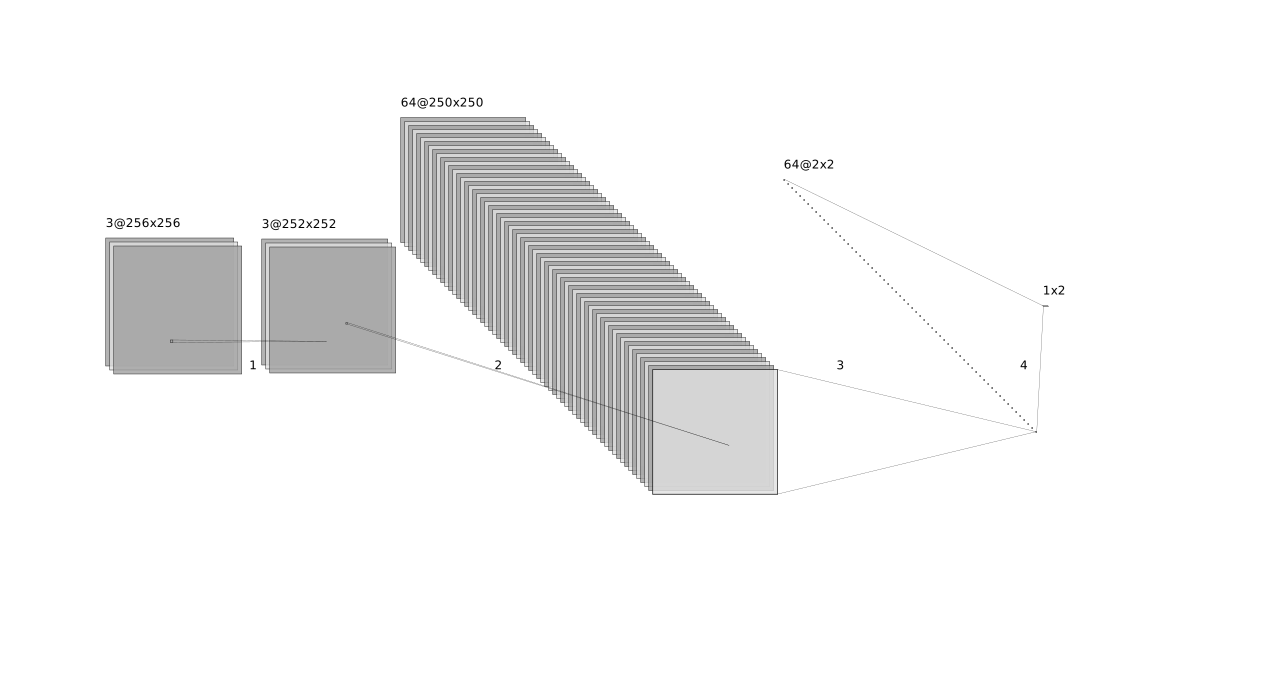
\includegraphics[width=1\textwidth]{include/graphics/mixed_color_architecture}
\caption{Архитектура комбинированной свёрточной сети}
\label{fig:ColorMixedCNNArchitecture}
\end{figure}

Для обучения GNCNN было использовано значение параметра $ \sigma $ функции активации, равное 0,1, и метод обучения Adam~\cite{Adam} со скоростью обучения 0,001, $ \beta_1 = 0,9 $, $ \beta_2 = 0,999 $. Для обучения нейронной сети с двумя свёрточными слоями и комбинированной нейронной сети использовался стохастический градиентный спуск со скоростью обучения 0,005.

Блок-схема работы комбинированной свёрточной сети показана на рисунке~\ref{fig:flowchart}.

\begin{figure}[ph]
\centering
\includegraphics[width=0.5\textwidth]{include/graphics/flowchart}
\caption{Блок-схема работы комбинированной свёрточной сети}
\label{fig:flowchart}
\end{figure}

\subsection{Цель, план и результаты эксперимента}

Целью проведения эксперимента было определение способности вышеописанных нейронных сетей различать пустые и заполненные различными стеганографическими методами контейнеры. Для заполнения использовалось следующее программное обеспечение:
\begin{itemize}
\item программная реализация метода создания цифровых водяных знаков на основе гетероассоциативных сжимающих преобразований (ГСП)~\cite{SirotaHIC},
\item собственная реализация метода относительной замены коэффициентов дискретного косинусного преобразования (ДКП) Коха и Жао~\cite{ZhaoKoch, KochZhao},
\item симулятор стеговстраивания с использованием алгоритма WOW~\cite{WOW}.
\end{itemize}

Выбор алгоритмов стеговстраивания обусловлен следующими предпосылками:
\begin{itemize}
\item метод создания цифровых водяных знаков на основе гетероассоциативных сжимающих преобразований (ГСП) является блочным, вносит малые искажения в контейнер и ранее не использовался в задачах стегоанализа с применением свёрточных нейронных сетей,
\item метод относительной замены коэффициентов дискретного косинусного преобразования (ДКП) Коха и Жао вносит существенные искажения и может служить индикатором общей работоспособности алгоритмов стегоанализа,
\item алгоритм WOW~\cite{WOW} не является блочным и признан среди современных стеганографических алгоритмов как один из наиболее скрытных.
\end{itemize}

Для проведения эксперимента использовалась база данных изображений PPG-LIRMM-COLOR~\cite{PPG-LIRMM-COLOR}, состоящая из 10 000 изображений в разрешении 512×512 пикселей. База данных подверглась конвертации в формат изображений в оттенках серого с помощью утилиты ppmtopgm~\cite{ppmtopgm}. Затем из каждого изображения были вырезаны два фрагмента размером 256×256 пикселей: один из них использовался для обучения нейронной сети сжатия в составе реализации метода создания цифровых водяных знаков на основе ГСП, второй – для осуществления встраивания обученной сетью. В дальнейшем последний фрагмент использовался для стеговстраивания с применением собственной реализации метода Коха и Жао, а также симулятора встраивания с использованием алгоритма WOW.

Таким образом, для обучения нейронных сетей были получены три выборки из 10 тыс. пустых и 10 тыс. заполненных одним из перечисленных стегоалгоритмов контейнеров в оттенках серого. Такие же выборки были получены для цветных изображений из оригинальной базы.

Ввиду отсутствия поддержки симулятором встраивания с использованием алгоритма WOW цветных изображений, пустые контейнеры предварительно были разделены по каналам цветности на три изображения, затем была произведена симуляция встраивания в изображения, соответствующие синем каналу, и наконец, разделённые изображения были вновь собраны в цветные заполненные контейнеры.

Кроме того, были сформированы аналогичные выборки из 1 тыс. пустых и 1 тыс. заполненных контейнеров для оценки влияния объёма выборки на точность классификации.

Обучающая подвыборка составила 90~\% полученной выборки, валидационная --- 10~\% во всех случаях.

В рамках эксперимента было произведено сравнение реализаций методов стеговстраивания по средней среднеквадратической ошибке и среднему проценту восстановленных посредством стегоизвлечения данных (таблица~\ref{table:1} для контейнеров в оттенках серого и таблица~\ref{table:1Color} для цветных), а также обучение рассмотренных нейронных сетей с целью оценки их способности к классификации стегоконтейнеров валидационной подвыборки (таблица~\ref{table:2} для контейнеров в оттенках серого и таблица~\ref{table:2Color} для цветных).

Для каждого стегоалгоритма указан параметр, характеризующий мощность стеговоздействия. Для метода на основе гетероассоциативных сжимающих преобразований им является амплитуда встраивания $ A_m $, для алгоритма Коха и Жао – разность между коэффициентами ДКП $ p $, кодирующая различие между логическими нулём и единицей встраиваемой битовой последовательности, для алгоритма WOW – количество встроенных битов, делённое на количество пикселей в изображении, $ \alpha $.

\begin{table}[h]
\centering
\caption{Сравнение методов встраивания в контейнеры в оттенках серого}
    \begin{tabular}{| l | l | l |}
    \hline
    Стегоалгоритм & MSE & Процент восстановленных данных \\ \hline
    На основе ГСП ($ A_m = 0,016 $) & 0,1334 & 97,23~\% \\ \hline
    Алгоритм Коха и Жао ($ p = 1 $) & 0,5775 & 99,78~\% \\ \hline
    WOW ($ \alpha = 0,4 $) & 0,0389 & – \\ \hline
%    \hline
    \end{tabular}
\label{table:1}
\end{table}

\begin{table}[h]
\centering
    \begin{tabular}{| l | l | l |}
    \hline
    Стегоалгоритм & MSE & Процент восстановленных данных \\ \hline
    На основе ГСП ($ A_m = 0,016 $) & 0.0475 & 98,79~\% \\ \hline
    Алгоритм Коха и Жао ($ p = 1 $) & 0.1995 & 99,76~\% \\ \hline
    WOW ($ \alpha = 0,4 $) & 0.0129 & – \\ \hline
%    \hline
    \end{tabular}
\caption{Сравнение методов встраивания в цветные контейнеры}
\label{table:1Color}
\end{table}

Процент успешно извлечённых после стеговстраивания данных для алгоритма WOW не указан ввиду использования симулятора, не производящего сокрытия информации, а лишь изменяющего пиксели соответственно алгоритму встраивания.
\begin{landscape}

\begin{table}[p]
\centering
    \begin{tabular}{| l | p{2cm} | p{2cm} | p{2cm} | p{2cm} | p{2cm} | p{2cm} |}
    \hline
    Стегоалгоритм & GNCNN (2 тыс.) & GNCNN (20 тыс.) & 2\=/хслойная НС (2 тыс.) & 2\=/хслойная НС (20 тыс.) & Комб. НС (2 тыс.) & Комб. НС (20 тыс.) \\ \hline
    На основе ГСП ($ A_m = 0,016 $) & 94,1~\% & 96,8~\% & 48~\% & 51,7~\% & 96~\% & 95,1~\% \\ \hline
    Алгоритм Коха и Жао ($ p = 1 $) & 50,7~\% & 93,1~\% & 100~\% & 99,8~\% & 100~\% & 99~\% \\ \hline
    WOW ($ \alpha = 0,4 $) & 50~\% & 49,6~\% & 85,5~\% & 96,3~\% & 92,5~\% & 95~\% \\ \hline
    \end{tabular}
\caption{Точность классификации контейнеров в оттенках серого}
\label{table:2}
\end{table}

\begin{table}[p]
\centering
    \begin{tabular}{| l | p{2cm} | p{2cm} | p{2cm} | p{2cm} | p{2cm} | p{2cm} |}
    \hline
    Стегоалгоритм & GNCNN (2 тыс.) & GNCNN (20 тыс.) & 2\=/хслойная НС (2 тыс.) & 2\=/хслойная НС (20 тыс.) & Комб. НС (2 тыс.) & Комб. НС (20 тыс.) \\ \hline
    На основе ГСП ($ A_m = 0,016 $) & 53,7~\% & 99,5~\% & 50~\% & 50~\% & 82,5~\% & 100~\% \\ \hline
    Алгоритм Коха и Жао ($ p = 1 $) & 49,3~\% & 49,1~\% & 99,5~\% & 100~\% & 98~\% & 98,1~\% \\ \hline
    WOW ($ \alpha = 0,4 $) & 50~\% & 49,4~\% & 54,5~\% & 96,7~\% & 90~\% & 91,1~\% \\ \hline
    \end{tabular}
\caption{Точность классификации цветных контейнеров}
\label{table:2Color}
\end{table}
\end{landscape}

Из таблицы~\ref{table:2} видно, что все три нейронные сети имеют практически одинаковую способность к различению пустых контейнеров и контейнеров, заполненных с применением метода Коха и Жао, на выборке из 20 тысяч изображений в оттенках серого.

Однако, нейронная сеть с двумя свёрточными слоями оказалась неспособна успешно детектировать контейнеры, заполненные с помощью метода на основе ГСП, а GNCNN --- заполненные с применением симулятора встраивания WOW, в то время как комбинированная свёрточная сеть одинаково хорошо справилась с обеими задачами.

Объём выборки не возымел существенного влияния на точность классификации во всех случаях, кроме распознавания контейнеров, заполненных методом Коха и Жао, нейронной сетью GNCNN.

Из таблицы~\ref{table:2Color} видно, что GNCNN распознаёт цветные контейнеры хуже, чем контейнеры в оттенках серого: для алгоритма на основе ГСП проявляется влияние объёма выборки, метод Коха и Жао перестаёт детектироваться вовсе. Различающая способность нейронной сети с двумя свёрточными слоями также начинает зависеть от объёма выборки для алгоритма WOW. Комбинированная свёрточная сеть ухудшает свои показатели по сравнению с результатами, полученными на выборке в оттенках серого, но точность классификации остаётся приемлемой.

Рисунки~\ref{fig:GrayscalePlotsHIC}--\ref{fig:ColorPlotsWOW} иллюстрируют процесс обучения нейронных сетей. На них изображены графики зависимости функции ошибок и точности классификации от количества эпох. Графики для тренировочной и валидационной подвыборок обозначены в легенде как <<training>> и <<validation>> соответственно. Помимо прочего, графики иллюстрируют более гладкий характер кривых для комбинированной свёрточной сети, обусловленный использованием $ L_2 $\=/регуляризации.

\begin{figure}[p]
    \centering

    \begin{subfigure}{\textwidth}
        \includegraphics[width=\textwidth]{include/graphics/experimental_plots/grayscale/gncnn_hic}
                    \caption{GNCNN}
    \end{subfigure}

    \begin{subfigure}{\textwidth}
        \includegraphics[width=\textwidth]{include/graphics/experimental_plots/grayscale/mixed_hic}
                    \caption{Комбинированная СНС}
    \end{subfigure}

   \caption{Графики процесса обучения для ГСП в оттенках серого}
    \label{fig:GrayscalePlotsHIC}
\end{figure}

\begin{figure}[p]
    \centering

    \begin{subfigure}{\textwidth}
        \includegraphics[width=\textwidth]{include/graphics/experimental_plots/grayscale/gncnn_koch}
                    \caption{GNCNN}
    \end{subfigure}

    \begin{subfigure}{\textwidth}
        \includegraphics[width=\textwidth]{include/graphics/experimental_plots/grayscale/mixed_koch}
                    \caption{Комбинированная СНС}
    \end{subfigure}

   \caption{Графики процесса обучения для Коха и Жао в оттенках серого}
    \label{fig:GrayscalePlotsKoch}
\end{figure}

\begin{figure}[p]
    \centering

    \begin{subfigure}{\textwidth}
        \includegraphics[width=\textwidth]{include/graphics/experimental_plots/grayscale/french_wow}
                    \caption{2-хслойная НС}
    \end{subfigure}
    ~
    \begin{subfigure}{\textwidth}
        \includegraphics[width=\textwidth]{include/graphics/experimental_plots/grayscale/mixed_wow}
                    \caption{Комбинированная СНС}
    \end{subfigure}

   \caption{Графики процесса обучения для WOW в оттенках серого}
    \label{fig:GrayscalePlotsWOW}
\end{figure}


\begin{figure}[p]
    \centering

    \begin{subfigure}{\textwidth}
        \includegraphics[width=\textwidth]{include/graphics/experimental_plots/color/gncnn_hic}
                            \caption{GNCNN}
    \end{subfigure}
    ~
    \begin{subfigure}{\textwidth}
        \includegraphics[width=\textwidth]{include/graphics/experimental_plots/color/mixed_hic}
                    \caption{Комбинированная СНС}
    \end{subfigure}

    \caption{Графики процесса обучения для цветного ГСП}
    \label{fig:ColorPlotsHIC}
\end{figure}

\begin{figure}[p]
    \centering

    \begin{subfigure}{\textwidth}
        \includegraphics[width=\textwidth]{include/graphics/experimental_plots/color/french_koch}
                            \caption{2-хслойная НС}
    \end{subfigure}
    ~
    \begin{subfigure}{\textwidth}
        \includegraphics[width=\textwidth]{include/graphics/experimental_plots/color/mixed_koch}
                    \caption{Комбинированная СНС}
    \end{subfigure}

    \caption{Графики процесса обучения для цветного Коха и Жао}
    \label{fig:ColorPlotsKoch}
\end{figure}

\begin{figure}[p]
    \centering

    \begin{subfigure}{\textwidth}
        \includegraphics[width=\textwidth]{include/graphics/experimental_plots/color/french_wow}
                                    \caption{2-хслойная НС}
    \end{subfigure}
    ~
    \begin{subfigure}{\textwidth}
        \includegraphics[width=\textwidth]{include/graphics/experimental_plots/color/mixed_wow}
                    \caption{Комбинированная СНС}
    \end{subfigure}

    \caption{Графики процесса обучения для цветного WOW}
    \label{fig:ColorPlotsWOW}
\end{figure}

\clearpage
